\newpage
\section{Objetivos}

Nessa prática, buscaremos determinar a densidade de líquidos e de sólidos, utilizando para isso, o princípio de Arquimedes (existência da força de empuxo, agindo sobre corpos imersos em fluidos).\\

Utilizando esses conceitos, conseguiremos determinar o volume de corpos desconhecidos - conhecendo suas massas-, e assim, calcular suas densidades.  \\

\begin{figure}[H]
    \centering
    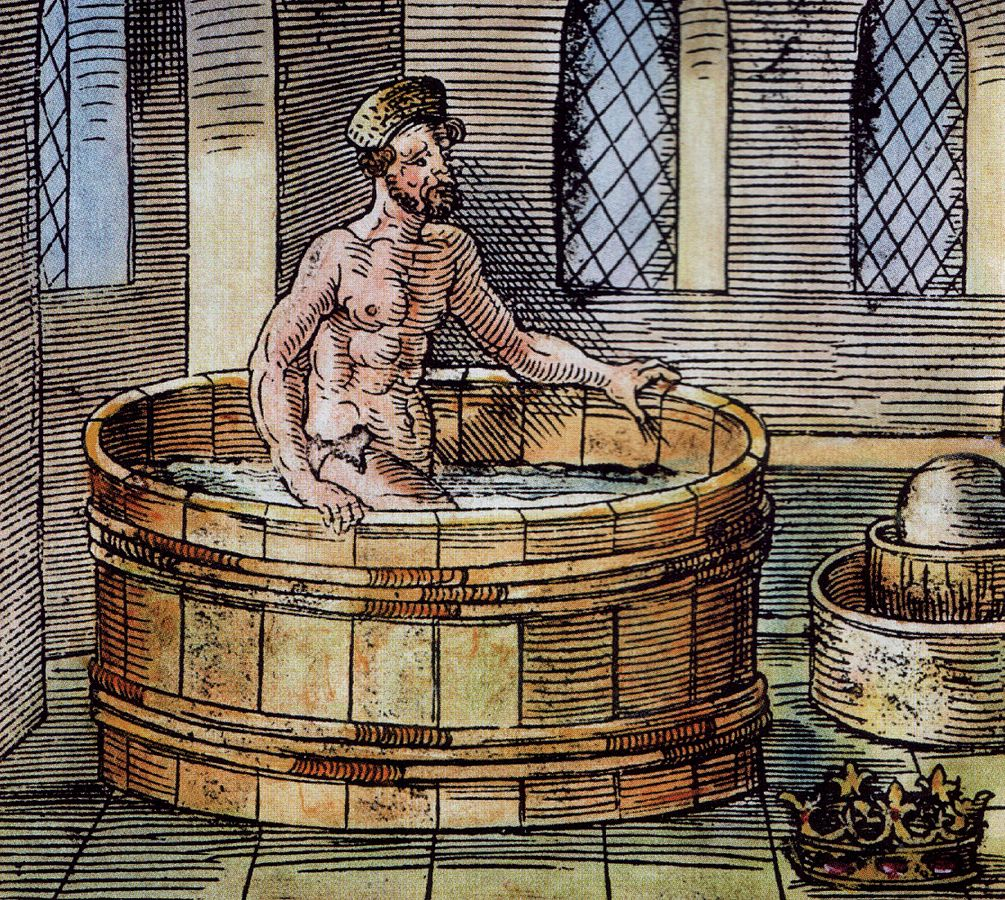
\includegraphics[scale=0.4]{images/Arquimedes.png}
    \caption{Ilustração de Arquimedes em sua icônica banheira}
\end{figure}

